%
\chapter{Implementation}\label{cha:Implementation}
%
\section*{3.1.Test Track}\label{sec:Test Track}
\addcontentsline{toc}{section}{3.1.Test Track}
%
\section*{3.2.Hardware}\label{sec:Hardware}
\addcontentsline{toc}{section}{3.2.Hardware}

%
\subsection*{3.2.1. Model Auto}\label{sec:Model Auto}
\addcontentsline{toc}{subsection}{3.2.1. Model Auto}
%

\subsection*{3.2.2. Microcontroller and Main Board}\label{sec:Microcontroller and Main Board}
\addcontentsline{toc}{subsection}{3.2.2. Microcontroller and Main Board}
%

\subsection*{3.2.3. Camera}\label{sec:Camera}
\addcontentsline{toc}{subsection}{3.2.3. Camera}

Camera is one of the main parts at lane detection and accordingly autonom driving. For this thesis, I had to search
the most suitable camera because all cameras have different properties. At the beginnig of the projectseminar 
"Echtzeitsysteme", Logitech C270 HD Webcam was being used. The resolation of the camera is 1280x960 pixels and the 
Frame per Second(FPS) value is 30 Hertz(Hz) at 640x480 pixels resolution. The field of View(FOV) is just 60 degree. The 
problem of this camera, if there is a curve, the camera can't see all of the lanes so this camera was not so suit for 
lane detection. When I started the master thesis, there was a Kinect v2 camera on the model car. Kinect v2 camera was 
developed by Microsoft and released in 2013. This camera has a depth sensor, resolution of which is 512x424 pixels and 
its FOV is 70x60 degree. The FPS value 30 Hz at 512x424 pixels resolution. This camera has also a color camera, 
resolution of which is 1920x1080 pixels and its FOV is 84.1x53.8 degree. The FPS value 30 Hz at 1920x1080 pixels 
resolution. This camera had 2 main disadvantages for this master thesis. The first disadvantage is the FOV value of 
camera. This value is better than the value of Logitech C270 camera but it is still not enough for curve lane detection.
The second main disadvantage is the location of color camera. The color camera of this camera is not at the middle of 
camera, it is on the right side of camera. This is a disadvantage for us because if the left going curves will come, the
camera can't see the left and maybe middle lane of the truck so it is a big problem in the lane detection.

Because of these reasons, I had to choose a camera which has enough high FOV value. After searching phase, I decided, 
that Genius Widecam F100 camera is the best choice for this master thesis, because this camera has FOV value 120 degree
and it can be used also at Linux Systems. Resolution of this camera is 1920x1080 pixels and FOV value is 120 degree.
The FPS is 30 Hz at 1920x1080 pixels resolution. With this camera, it is mostly possible to detect all lanes also at
curves. 

\begin{figure}
	\centering
	\hspace*{0cm}   
	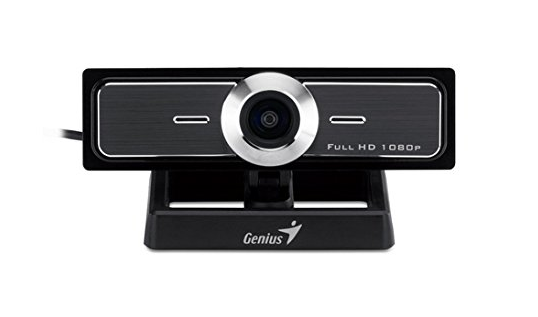
\includegraphics[width=150mm,scale=1]{./Bilder/Genius_F100_camera.png}
	\caption{Genius 120-degree Ultra Wide Angle Full HD Conference Webcam(WideCam F100) }
\end{figure}


%
\section*{3.3.Software}\label{sec:Software}
\addcontentsline{toc}{section}{3.3.Software}
%


